\documentclass[a4paper, 12pt]{article}
\usepackage{geometry}
\geometry{margin=1in}
\usepackage{amsmath, amssymb}
\usepackage{graphicx}
\usepackage{natbib}
\usepackage{setspace}
\doublespacing
\setlength{\parindent}{15pt}
\setlength{\parskip}{0pt}
\usepackage[hidelinks]{hyperref}
\usepackage{tikz}
\usepackage[affil-it]{authblk}
\usepackage{tabularx}
\usepackage{booktabs}  % For cleaner table lines
\usepackage{threeparttable}
\usetikzlibrary{arrows.meta, positioning}
\onehalfspacing
\usepackage[table]{xcolor}
\usepackage{dcolumn}
\usepackage{appendix}
\usepackage{float}
\usepackage{pdflscape}

\title{Longer Exposure, Better Outcomes: Evidence from Indonesia’s BOS Program}
\author{Gregy Tuerah}
\date{}

\begin{document}

\maketitle

\begin{abstract}
This thesis studies whether Indonesia's \textit{Bantuan Operasional Sekolah} (BOS) program improved educational attainment by reducing the recurring cost burden of schooling. BOS was introduced in 2005 as a national school operational grant intended to support school operating costs and reduce routine charges faced by households in basic education. Using data from the Indonesia Family Life Survey (IFLS), I compare siblings within the same origin household who differed in potential BOS exposure because of their birth cohort. I combine this within-household cohort variation with cross-province variation in a BOS-related implementation-intensity proxy constructed from the 2007 IFLS school-facility data.

One additional year of potential BOS exposure is associated with about a 1 percentage point increase in the probability of reaching senior high school in higher-intensity provinces relative to lower-intensity provinces. Among higher-exposure children in the analytic sample, the median child had six potential BOS-exposed school years; at that level of exposure, the preferred estimate implies roughly a 6 percentage point higher probability of senior-high attainment. The estimates for completed years of schooling are weaker and less stable. Taken together with three sensitivity checks, the results provide suggestive causal evidence that BOS supported progression to senior high school where implementation intensity was stronger, while also highlighting the need for richer administrative data on BOS disbursement and execution.

\end{abstract}


\section{Introduction}
\begin{doublespacing}
Education is one of the central ways individuals accumulate human capital and improve long-run economic opportunities. Across countries, and especially in developing-country settings, a large literature links schooling to higher earnings and improved labor-market outcomes \citep{PsacharopoulosPatrinos2018,Duflo2001,Delesalle2021}. For this reason, education policy remains a core component of development strategy \citep{HanushekWoessmann2007,GlewweMuralidharan2016}. Those returns, however, depend not only on whether children ever enroll in school, but also on whether they progress far enough for schooling to translate into completed educational attainment.

This creates a policy problem that is especially important in developing-country settings: even when primary and junior-secondary schooling are nominally free or heavily subsidized, families may still face registration costs, learning materials, transportation, uniforms, examination fees, and the opportunity cost of children's time \citep{GlewweMuralidharan2016,DufloDupasKremer2021}. These constraints often become more important at later grades, when continuation decisions are more sensitive to costs and competing household demands \citep{FilmerSchady2014,DufloDupasKremer2021}. The senior-high transition is therefore a useful policy margin: it asks whether a school-finance intervention helps children move beyond the basic-education cycle, not merely whether they enroll at earlier grades.

Indonesia provides an especially useful setting for studying how large-scale education policy affects progression beyond basic schooling. The country has a long history of large-scale education interventions. Most notably, \citet{Duflo2001} studies the INPRES primary school construction program and shows that school construction increased schooling and wages among cohorts exposed during primary-school age. That evidence established Indonesia as a foundational case for cohort-based education-policy evaluation. Beginning in the mid-2000s, however, the policy focus shifted from building schools toward reducing the recurring costs of schooling. The major intervention in this period was the \textit{Bantuan Operasional Sekolah} (BOS) program, introduced in 2005.

BOS provides operational grants to schools and is intended to reduce the education-cost burden on households, especially at the primary and junior-secondary levels. In practice, the program was designed to support school operations, reduce or eliminate routine tuition-related charges in basic education, and finance operating needs such as learning materials \citep{WorldBank2008,UNESCOIIEPUNICEF2016}. Existing evidence suggests that BOS can relax household budget constraints and improve some schooling outcomes, but it also shows that the subsidy does not necessarily eliminate all education costs. \citet{Sulistyaningrum2016} finds positive effects on student performance using propensity-score matching, while \citet{SariTanaka2019} finds that BOS increased household educational investment, especially among lower-income households. Related IFLS-based evidence finds that school-level BOS implementation increased senior-secondary enrollment \citep{KartasasmitaSulistyaningrum2021}, and other DiD-style studies examine BOS effects on dropout and the transition from primary to junior secondary school \citep{Kharisma2018,KharismaRemiMaharani2021}.

This thesis studies BOS by using sibling-level variation in potential exposure. Rather than comparing unrelated children or households, I compare children from the same origin household who were different ages when BOS began. Younger siblings were still between ages 6 and 15 for more years after the 2005 rollout, so they had more potential school-age exposure to BOS than older siblings. I then examine whether this within-family exposure difference is associated with larger educational gains in provinces where measured BOS implementation intensity was higher. The design is closely related to the cohort-exposure by regional-intensity logic in \citet{Duflo2001}, but applies it to a household fixed-effects setting.

\textbf{The core research question of this thesis is: within the same family, do children with greater potential exposure to Indonesia's BOS program attain more schooling and have a higher probability of reaching senior high school than their less-exposed siblings, especially in provinces with stronger measured BOS intensity?}

This question is motivated by the broader literature on family background, sibling differences, and educational attainment. Children who share the same household may still differ in realized educational outcomes because of birth order, sibling composition, parental investments, and household constraints \citep{BlackDevereuxSalvanes2005,NicolettiRabe2019,FerreiraSandholtz2024}. I do not directly observe how families reallocate resources across children after BOS. Instead, the sibling comparison is used as an identification strategy: household fixed effects absorb stable family-level characteristics, while birth-cohort differences generate variation in potential BOS exposure within the same family.

The main outcome is senior-high attainment, defined as having completed at least 10 years of schooling. This outcome captures progression into the senior-secondary stage and is more closely aligned with the policy margin where cost constraints may still bind. Completed years of education is retained as a secondary outcome, but it is less central because completed schooling remains mechanically linked to age in the 2014 cross-section.

The main findings are modest but informative. In the preferred household fixed-effects specification, one additional potential BOS-exposed school year in a high-intensity province is associated with about a 1 percentage point higher probability of reaching senior high school. This per-year estimate sounds small in isolation, but exposure accumulates across school years. Among higher-exposure children in the analytic sample, the median child had six potential BOS-exposed school years. Multiplying the preferred estimate by this exposure level implies about a 6 percentage point higher probability of senior-high attainment in higher-intensity provinces relative to lower-intensity provinces, or roughly 10 percent of the control-group mean of 0.618. By contrast, the estimates for completed years of education are weaker and not robust across specifications. The value of this result is therefore not only its magnitude, but also the way it identifies the margin at which BOS may have mattered: cumulative exposure in places where the program appears to have been implemented more intensively.

This framing leads to three contributions. First, this thesis contributes to the BOS evaluation literature by changing both the comparison group and the treatment margin. Existing BOS studies already provide useful empirical evidence, including matching-based estimates of student performance and senior-secondary enrollment, household-level evidence on education spending, and DiD-style\footnote{Kharisma (2018) and Kharisma et al. (2021) used this DiD style method. I cite their studies as part of the BOS evidence base rather than as definitive causal benchmarks. Their designs rely on broad before-after survey comparisons, so the parallel-trends and counterfactual assumptions are difficult to verify.} estimates of dropout or school-transition outcomes \citep{Sulistyaningrum2016,SariTanaka2019,KartasasmitaSulistyaningrum2021,Kharisma2018,KharismaRemiMaharani2021}. These studies generally evaluate average differences associated with BOS receipt, school-level implementation, or program exposure. This thesis instead compares siblings within the same origin household and measures exposure as the number of potential BOS-exposed school years. The continuous exposure measure makes the preferred estimate interpretable per additional exposed school year and allows the result to be scaled to longer exposure windows, which is closer to how a national program affects cohorts as they pass through multiple grades.

Second, this thesis connects the BOS literature to research on sibling differences and intra-household allocation. Recent evidence shows that families may allocate time and material resources unevenly across siblings, with meaningful differences emerging even among children who share the same household environment \citep{Kirchberger2020}. Related work also shows that birth order and family structure are systematically associated with children's educational attainment, suggesting that parental investments are not distributed uniformly across children \citep{DeHaan2010,BaggerEtAl2021}. This thesis does not directly observe parental resource allocation, but it brings the sibling perspective into the evaluation of Indonesia's largest school subsidy program by studying whether siblings with different potential exposure to BOS reach different educational outcomes.

Third, this thesis contributes to the evaluation of long-running education policies in Indonesia. Although BOS has operated since 2005 and remains one of the country's central school-financing programs, policy reviews continue to emphasize that its effectiveness depends on implementation quality, fund disbursement, local oversight, and administrative capacity \citep{WorldBank2014,SMERUUNESCO2024}. This continuing need for evaluation is especially important because Indonesia's education challenge has increasingly shifted from expanding access alone toward improving progression, quality, and learning. In this sense, the thesis provides new evidence on a continuing policy while also motivating future work using richer administrative data and longer-run program measures.

The policy implication is direct: if BOS affects educational progression, it appears to do so more strongly where implementation intensity is greater. This pattern is consistent with policy reviews emphasizing that the practical performance of BOS depends on disbursement timing, administrative capacity, local oversight, and school-level implementation, not only on the national allocation rule \citep{WorldBank2008,WorldBank2014,SMERUUNESCO2024}. Improving implementation quality may therefore be as important as changing the nominal scale of the subsidy.

The remainder of the thesis proceeds as follows. Chapter 2 reviews the historical development of Indonesia's education system and the institutional background of BOS. Chapter 3 discusses the data, treatment measurement, identification strategy, and empirical methodology. Chapter 4 presents the main results, heterogeneous treatment effects, and sensitivity checks. Chapter 5 discusses policy implications and limitations. Chapter 6 concludes.


\section[Background: Historical development of Indonesia's education landscape]{Background: Historical development of \\ Indonesia's education landscape}
\subsection{Before BOS}
Indonesia's education system has undergone repeated institutional and policy reforms as the government shifted from expanding access at the primary level to improving participation and progression in secondary education. Formal schooling is organized into primary education, junior secondary education, senior secondary education, and higher education. Basic education consists of six years of primary school and three years of junior secondary school, followed by three years of senior secondary education \citep{WorldBank2013}.\footnote{In the Indonesian system, primary school generally covers grades 1--6, junior secondary covers grades 7--9, and senior secondary covers grades 10--12. During the period studied here, the compulsory basic-education cycle covered primary and junior secondary schooling.} This thesis focuses on formal schooling up to the senior-secondary level.

A major turning point in the expansion of Indonesian schooling occurred during the New Order period, when the government used oil revenues to finance large-scale public investment in infrastructure, including education. One of the most important initiatives was the Sekolah Dasar INPRES primary school construction program. As \citet{Duflo2001} documents, this was one of the largest school-construction efforts ever undertaken, and the number of schools allocated across districts was tied to the number of primary-school-age children who were not enrolled in school. The program substantially expanded access to primary schooling and helped Indonesia move toward near-universal primary enrollment \citep{Duflo2001,WorldBank2013}.

Once access to primary schooling had expanded, policy attention shifted from school construction toward completion and progression. In 1984, the government made six years of primary education compulsory. In 1994, compulsory basic education was extended from six to nine years, reflecting a broader policy shift toward increasing participation in junior secondary school and improving progression beyond the primary level \citep{WorldBank2013}. Earlier work on Indonesia's education investment priorities also emphasized that expanding junior secondary education offered high social returns, reinforcing the importance of progression through grade 9 \citep{McMahonBoediono1992}. By that stage, the central challenge in Indonesian education was no longer simply whether children entered school, but whether they progressed through the full cycle of basic education.

Despite these access gains, continued participation beyond primary school remained uneven. The World Bank's education-sector reviews emphasize that transition into and completion of secondary schooling continued to vary across regions and socioeconomic groups \citep{WorldBank2013}. Household costs remained part of this problem. Before BOS, households still faced school fees, contributions, books, uniforms, transportation, examination fees, and other education-related expenses. In the BOS-KITA review, \citet{WorldBank2008} reports that among households in the poorest quintile, 34 percent with primary-school children and 44 percent with junior-secondary children reported difficulty financing school fees. Cost barriers therefore remained relevant even after Indonesia had expanded the physical supply of schools.

A second major turning point came with decentralization. Laws 22 and 25 of 1999 transferred substantial political and fiscal authority to districts and municipalities beginning in 2001, including important responsibilities related to education governance and service delivery \citep{Bjork2004}. In the education sector, this meant that subnational governments took on a much larger role in the organization and management of primary and secondary schooling, while the central government retained authority over national policy, standards, and the overall framework of the system \citep{Bjork2004,WorldBank2013}. Although decentralization was intended to improve responsiveness and efficiency, it also created new challenges of coordination, financing, and accountability across levels of government.

This institutional context helps explain the emergence of BOS. Once Indonesia had largely expanded physical access to schooling and extended compulsory education to nine years, the next policy challenge was to reduce the recurring cost burden that still prevented many children from remaining in school. After decentralization, a centrally financed but school-directed grant mechanism offered a way to support school operations, lower household cost burdens, and strengthen school-based management without reversing the broader decentralized structure of education governance \citep{Bjork2004,WorldBank2008}.

\subsection{Introduction of BOS}
The \textit{Bantuan Operasional Sekolah} (BOS) program was introduced in July 2005 as a national school grant program intended to reduce the cost of basic education for households while supporting the operational needs of schools. BOS was introduced in the context of the government's 2005 fuel-subsidy reforms, when part of the compensation package was redirected toward social-sector programs, including education support \citep{IsdijosoEtAl2006}. In this sense, BOS represented a shift in Indonesian education policy away from school construction as the main instrument of access expansion and toward reducing the recurrent costs that constrained schooling continuation.

The program was large from the beginning. Table \ref{tab:bos_allocation} summarizes BOS allocation and coverage during the first three years of the program. In 2005, BOS covered nearly 40 million students and accounted for 18 percent of the central education budget. By 2006 and 2007, its share of the central education budget had increased to 23 percent \citep{WorldBank2008}. This scale is important for the thesis because BOS was not a small pilot program. It was a national school-finance reform large enough to plausibly affect the household cost environment faced by school-age children.

\begin{table}[H]
\caption{BOS allocation and program coverage, 2005--2007}
\label{tab:bos_allocation}
\centering
\begin{threeparttable}
\begin{tabular}[t]{lrrr}
\toprule
Year & 2005 & 2006 & 2007 \\
\midrule
Number of students (millions) & 39.63 & 39.92 & 39.51 \\
BOS allocation, nominal (US\$ billion) & 0.56 & 1.13 & 1.30 \\
BOS allocation, real (2006 = 100, US\$ billion) & 0.64 & 1.13 & 1.22 \\
BOS share of central education budget (\%) & 18 & 23 & 23 \\
\bottomrule
\end{tabular}
\begin{tablenotes}[para]
\item \textit{Note:} Source: \citet{WorldBank2008}. BOS share reports BOS spending as a share of the central education budget. In 2005, BOS accounted for 18 percent of the central education budget, or roughly 2.5 percent of the national budget.
\end{tablenotes}
\end{threeparttable}
\end{table}


A defining feature of BOS was its allocation mechanism. Unlike earlier funding arrangements that were often more fragmented and less transparent, BOS disbursed block grants to schools using a simple per-student formula \citep{WorldBank2008}. Funding was directly tied to student enrollment, which created a transparent rule for allocating school operational support. Although the program was centrally designed, funds were transferred to school accounts through provincial BOS teams, giving schools direct access to operational resources and greater discretion in day-to-day spending. As noted by \citet{WorldBank2008}, this made BOS one of the most important reforms in Indonesian education financing because grants were both formula-based and directly channeled to schools.

The direct purpose of BOS was to reduce the cost burden of basic education, but it did so through schools rather than through cash transfers to households. The program was designed to finance non-salary operating expenses so that schools would have less need to charge households for routine operating costs. The BOS operations manual also allowed schools to use funds for a broad set of operational purposes, including learning materials, maintenance, examinations, transportation support for poor students, and support for poor students' school supplies \citep{WorldBank2008,UNESCOIIEPUNICEF2016}. In this sense, BOS was not only a tuition-fee policy. It was a school operational grant intended to reduce school charges and strengthen the everyday financing of basic education.

Available implementation evidence suggests that BOS did reduce fees, but not always one-for-one with the value of the grant. The BOS-KITA review reports that school fees fell by 37 percent in primary schools and 39 percent in junior-secondary schools in real terms after BOS. It also reports that 88 percent of school committees said poor students had been released from various school fees and charges, while 76 percent reported that all students in their schools had been exempted from all school fees and charges \citep{WorldBank2008}. At the same time, BOS became the largest source of discretionary non-salary operational funding at the school level, representing more than 75 percent of non-salary operational resources \citep{WorldBank2008}. Later World Bank analysis similarly finds that the introduction of BOS was associated with an initial decline in household education spending, especially among poorer households and in government schools, but that the decline was small relative to the size of the per-student grants received by schools \citep{WorldBank2014}. This pattern is important for the thesis: BOS plausibly reduced the cost burden faced by households, but part of the grant also financed school operations rather than directly lowering every cost paid by families.

This mixed implementation pattern is consistent with the program's design. BOS was expected to reduce or waive routine charges, especially for poor students, but schools still had discretion over how to use funds within authorized categories. Moreover, grant guidelines allowed some parental contributions for costs not met by government funding, and later policy reviews continued to document disbursement delays, uneven information, weak monitoring, and limited parental participation \citep{UNESCOIIEPUNICEF2016,WorldBank2014,SMERUUNESCO2024}. The empirical question is therefore not whether BOS mechanically eliminated all schooling costs. It is whether greater potential exposure to BOS, especially in places where implementation intensity was stronger, is associated with higher educational attainment.

The funding formula also helps explain why realized BOS support could vary across schools and regions. At the most basic level, schools with larger enrollments received larger grants because BOS was allocated on a per-student basis. In addition, the per-student amount differed by level of schooling, with junior secondary schools receiving more per student than primary schools \citep{IsdijosoEtAl2006,WorldBank2008}. The central BOS team prepared budget allocations using enrollment data reported through district and provincial management teams, while provincial BOS teams executed transfers to school bank accounts. District BOS teams compiled and verified enrollment data, supervised implementation, and handled monitoring and complaints \citep{WorldBank2008}. As a result, realized implementation depended not only on the national formula, but also on enrollment reporting, administrative verification, school-level uptake, and local execution.

This distinction is important for the empirical design. The national BOS rule was formula-based, but implementation in the field could still vary because execution depended on local administrative processes and school-level use of operational support.\footnote{Early implementation evidence is consistent with these frictions. \citet{IsdijosoEtAl2006} report that some schools refused BOS funds, that many implementers had insufficient understanding of the operational guidelines because socialization was weak, and that some funds remained uncollected by non-participating schools. Later qualitative work documents delayed disbursement, weak supervision, limited parental participation, and uneven information about BOS and its reporting at the school level \citep{UNESCOIIEPUNICEF2016,SMERUUNESCO2024}. World Bank reviews also note that school committees were often only weakly involved in decisions over BOS fund allocation \citep{WorldBank2014}.} The IFLS does not provide complete administrative BOS disbursement histories for each child's school, so Chapter 3 uses school-reported BOS-related operational funding in the IFLS school module to proxy for cross-province differences in realized BOS implementation intensity.

\section{Research Design and Empirical Strategy}
\subsection{Identification Strategy and Estimating Equation}
This thesis estimates the relationship between potential exposure to Indonesia's School Operational Assistance program (BOS) and educational attainment using a within-family cohort-exposure by regional-intensity design that follows the empirical logic of \citet{Duflo2001}. The design can be understood as a generalized difference-in-differences strategy. The first comparison is within the same origin household: younger siblings had more potential BOS exposure than older siblings because a larger share of their school-age years occurred after BOS began in 2005. The second comparison is across provinces: the within-household exposure difference is allowed to vary with the measured intensity of BOS-related school funding in the province.

The main empirical specification is a linear model with origin-household fixed effects estimated on the 2014 cross-section:

\begin{equation}
    Y_{ih} = \beta_{1} Exposure_{i} + \beta_{2} \left(Exposure_i \times Intensity_{r, 2007}\right) + X'_{i}\gamma + \alpha_h  + \varepsilon_{ih},
\end{equation}

where $Y_{ih}$ denotes the educational outcome of child $i$ in origin household $h$, $Exposure_{i}$ is either the binary higher-exposure cohort indicator or the continuous count of potential BOS-exposed school years, $Intensity_{r, 2007}$ is either the continuous 2007 province BOS intensity proxy or the binary high-intensity indicator, $X_{i}$ is a vector of child-level controls, $\alpha_{h}$ denotes origin-household fixed effects, and $\varepsilon_{ih}$ is an idiosyncratic error term. Because the regional intensity measure is constant within household in the 2014 cross-section, its standalone main effect is absorbed by household fixed effects and is not separately identified.

The coefficient of interest is $\beta_{2}$, the interaction between potential BOS exposure and province-level BOS intensity. In the preferred specification, exposure is measured as the number of potential BOS-exposed school years and intensity is measured as an indicator for provinces above the median of the 2007 intensity distribution. This coefficient captures whether the within-household relationship between BOS exposure and educational attainment is more positive in provinces with stronger measured BOS implementation intensity.

I do not observe the exact BOS disbursement history for each child's school over the full childhood period. For that reason, the treatment variable should be interpreted as potential exposure based on birth cohort and policy timing, not as verified individual receipt of BOS funds. The estimates are therefore causal estimates for the cohort-exposure by intensity comparison defined in the research design, rather than estimates of the effect of a precisely observed rupiah amount received by a specific school.

The identifying assumption is that, conditional on origin-household fixed effects and observed child characteristics, within-household differences in educational attainment between more-exposed and less-exposed siblings would not have been systematically larger in higher-intensity provinces for reasons unrelated to BOS. Origin-household fixed effects absorb all time-invariant characteristics shared by siblings within the same family, including persistent socioeconomic background, parental preferences, and other household-level factors that could otherwise confound comparisons across households \citep{AngristPischke2009}. Standard errors are clustered at the origin-household level to account for within-household correlation in the residuals.

\subsection{Data and Sample Construction}
The analysis combines child-level and household-level data from the Indonesia Family Life Survey (IFLS) with school-facility data from the IFLS community and school modules for the 2007 and 2014 survey rounds. The individual and household files are used to construct birth year, sibling structure, educational outcomes, and household characteristics, while the school-facility files are used to construct the regional BOS intensity measure. The relevant family unit for sibling comparisons is the origin household.

The main reported regressions use one observation per child from the 2014 IFLS wave. Earlier survey waves are used only to harmonize variables, define origin-household sibling groups, and construct pre-determined covariates and the 2007 BOS intensity measure. After requiring non-missing outcome and intensity data, the 2014 estimation sample contains 2,112 children from 915 origin households. The household fixed-effects estimator then drops a small number of singleton observations, leaving 2,088 children in the cleaned main regression tables. These singleton observations are children from origin households that contribute only one usable child to the 2014 fixed-effects estimation sample, so they do not identify within-household differences.

\begin{table}[!htbp]
\caption{Balance by Birth Cohort: Lower-Exposure (1988--1992) vs. Higher-Exposure (1994--1997)}
\label{tab:balance}
\centering
\vspace{-0.5em}
\begin{threeparttable}
\small
\setlength{\tabcolsep}{3pt}
\renewcommand{\arraystretch}{0.95}
\begin{tabular}[t]{@{}lrrrrr@{}}
\toprule
Variable & Lower exposure & Higher exposure & Diff. & p-value & Norm. diff.\\
\midrule
Children (N) & 1095 & 1017 &  &  & \\
\addlinespace
\multicolumn{6}{l}{\textit{Panel A. Baseline covariates}}\\
Female & 0.470 & 0.483 & 0.012 & 0.567 & 0.025\\
Urban & 0.443 & 0.456 & 0.013 & 0.539 & 0.027\\
Log per-capita exp. & 12.765 & 12.780 & 0.015 & 0.596 & 0.024\\
HH size & 6.373 & 6.354 & -0.019 & 0.836 & -0.009\\
Female-headed HH & 0.113 & 0.113 & -0.000 & 0.997 & -0.000\\
Max parent educ. & 7.985 & 8.092 & 0.107 & 0.568 & 0.025\\
\addlinespace
\multicolumn{6}{l}{\textit{Panel B. Design variables}}\\
BOS intensity share & 0.247 & 0.245 & -0.001 & 0.796 & -0.011\\
High intensity & 0.535 & 0.525 & -0.010 & 0.643 & -0.020\\
\bottomrule
\end{tabular}
\vspace{-0.4em}
\begin{tablenotes}[para]
\item \textit{Note: }
\item The lower-exposure group includes children born in 1988--1992; the higher-exposure group includes children born in 1994--1997. The table is restricted to children in the 2014 analytic sample before household fixed-effects singleton observations are dropped. Panel A reports predetermined child and household covariates measured in 2007. Panel B reports design variables based on the 2007 province-level BOS intensity proxy. BOS intensity is the province share of sampled IFLS schools reporting positive BOS-related local operational funding in 2007. High intensity equals one for provinces above the 2007 median of this proxy. p-values come from two-sided t-tests of equality in group means. Age is omitted because treatment status is mechanically defined by birth year.
\end{tablenotes}
\end{threeparttable}
\end{table}


Table \ref{tab:balance} reports baseline balance between the lower-exposure and higher-exposure birth cohorts using pre-determined household and child characteristics measured in 2007. The table is restricted to the 2,112 children in the 2014 analytic sample before household fixed-effects singleton observations are dropped: 1,095 children born in 1988--1992 and 1,017 children born in 1994--1997. Reassuringly, the cohort groups look very similar on gender composition, urban residence, log per-capita expenditure, household size, female headship, maximum parental education, and the two BOS intensity measures. The p-values from two-sided t-tests are all well above conventional significance levels, meaning that I do not reject equality of means between the lower- and higher-exposure cohorts for any reported baseline characteristic.\footnote{In this context, a p-value above 0.05 means the observed difference is not statistically distinguishable from zero at the 5 percent level. It should not be read as proving that the two cohort groups are identical, nor does it rule out differences in unobserved characteristics.} All normalized differences\footnote{Following \citet{ImbensWooldridge2009}, the normalized difference is a scale-free balance metric that expresses the difference in group means relative to the pooled dispersion of the covariate. Unlike a conventional difference-in-means test, it is not mechanically driven by sample size, so it is more informative for assessing substantive covariate balance across groups. As a practical rule of thumb, values below about 0.25 are typically viewed as indicating acceptable balance.} are also far below conventional imbalance thresholds. Taken together, these diagnostics support the interpretation that the main identifying variation comes from cohort exposure interacted with BOS intensity rather than from large observed baseline compositional differences across the analytic cohorts.


Figure \ref{fig:sample_map} shows the geographic distribution of origin households in the analytic sample. The sample is concentrated in the IFLS provinces on Java and Sumatra, with especially large numbers of origin households in West Java, Central Java, East Java, and North Sumatra, but it also includes observations from several provinces outside the core western-island concentration. This spatial coverage is useful for the empirical design because the BOS intensity proxy is defined at the province level. At the same time, the map also makes clear that the sample is not nationally uniform, which is one reason the results should be interpreted as evidence for the IFLS analytic sample rather than for the full Indonesian population.

\begin{figure}[H]
\centering
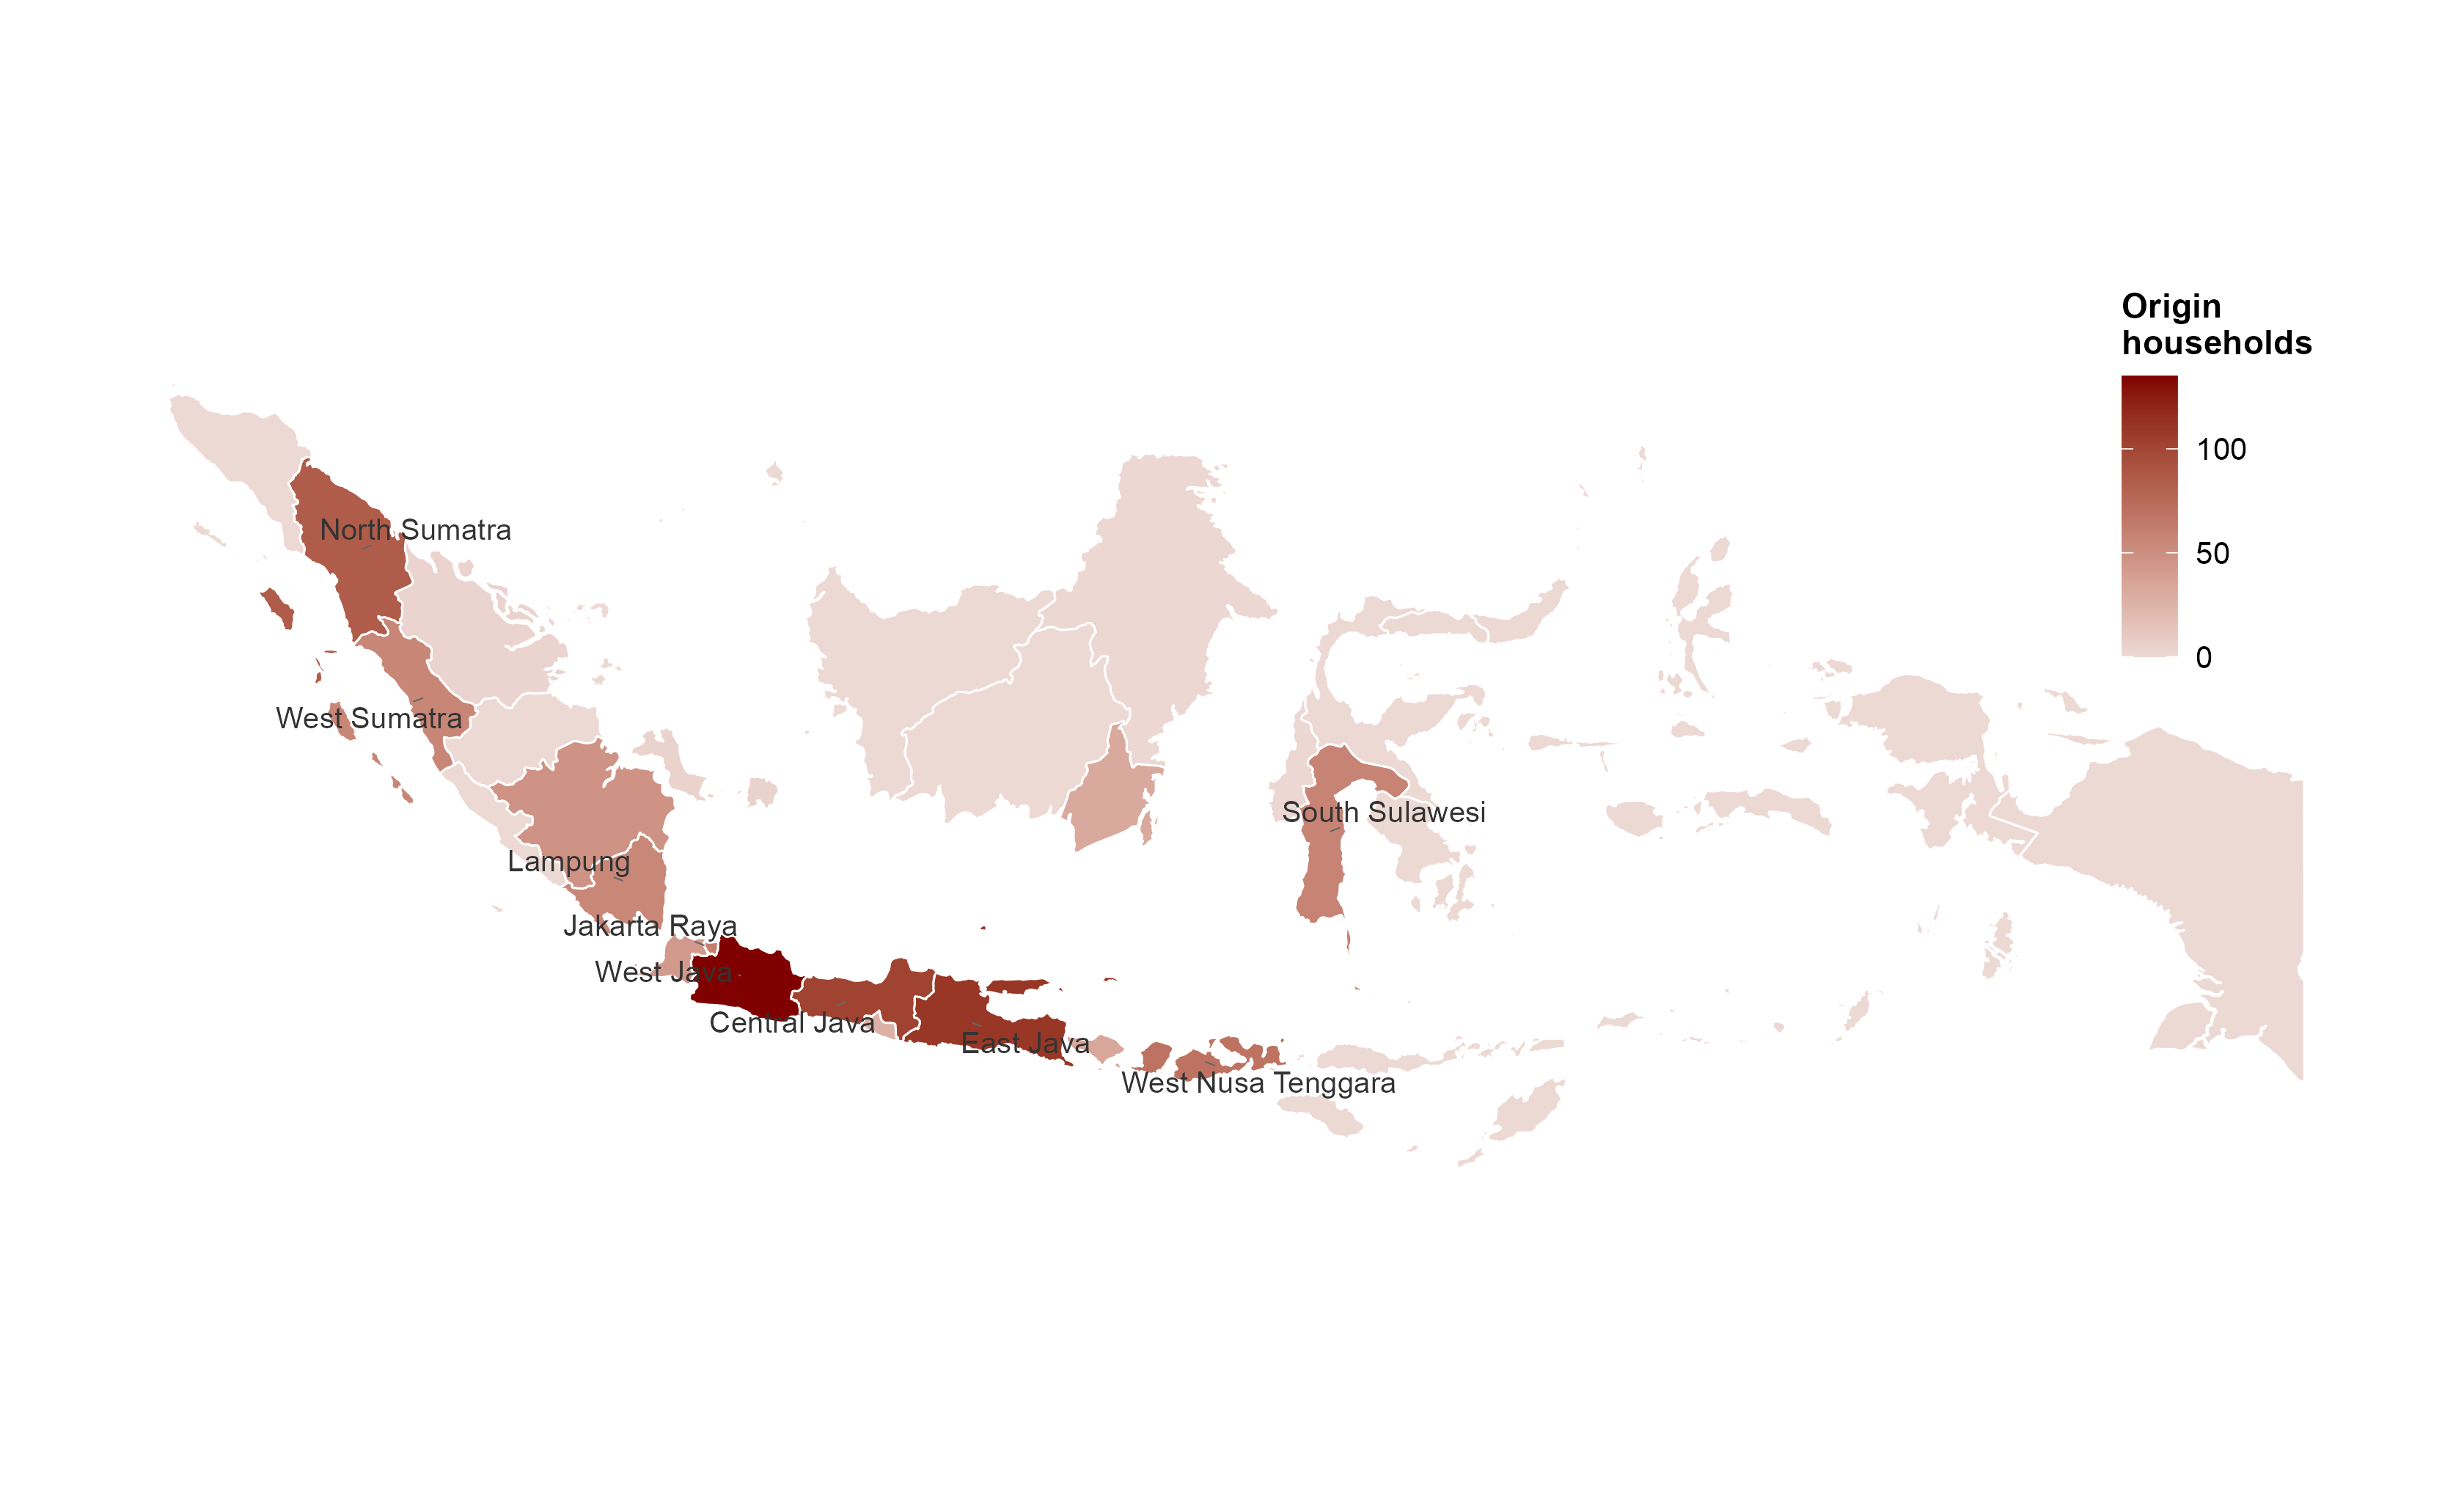
\includegraphics[width=0.95\textwidth]{indonesia_sample_origin_province_map_r.png}
\caption{Geographic Distribution of Origin Households in the Analytic Sample}
\label{fig:sample_map}
\end{figure}

The primary outcome is a senior-high attainment indicator equal to one if completed years of schooling are at least 10. This measure captures whether a child has crossed the senior-high threshold in terms of completed attainment. It is used as the main binary outcome because it is directly policy-relevant and less mechanically tied to age than continuous completed schooling. The secondary outcome is completed years of schooling.

\subsection{Treatment Measurement}
The first treatment dimension is BOS exposure. Exposure is defined from the timing of the BOS policy and each child’s birth year. Because the program began in 2005, children from different cohorts experienced different potential exposure depending on how many of their school-age years occurred after the program started. I classify children born between 1988 and 1992 as the lower-exposure cohort and children born between 1994 and 1997 as the higher-exposure cohort, excluding the 1993 transition cohort. In addition to this binary cohort indicator, I construct a continuous exposure measure equal to the number of potential BOS-exposed school years between ages 6 and 15 implied by each child’s birth year and the 2005 policy rollout.

The second treatment dimension is regional BOS intensity. In the main specification, intensity is measured using the 2007 IFLS school-facility file. I extract school-level information on BOS-related local operational funding, clean IFLS sentinel and missing values, define an indicator for whether a sampled school reports positive BOS-related local operational funding, and aggregate this measure to the province level. The continuous intensity proxy is therefore the 2007 province share of sampled schools reporting positive BOS-related local operational funding. I also construct a binary high-intensity measure equal to one for provinces above the median of the 2007 intensity distribution.

Figure \ref{fig:intensity_map} maps this province-level 2007 BOS intensity proxy. Darker provinces have a larger share of sampled schools reporting positive BOS-related local operational funding. This measure should be interpreted as a proxy for realized implementation intensity, not as a direct observation of the official BOS allocation formula or of the exact amount received by each child's school. It is motivated by the fact that the BOS allocation rule was national and formula-based, but execution in the field could still differ because of enrollment reporting, verification, and local administrative implementation. Using the 2007 measure also helps keep the intensity proxy pre-determined relative to the 2014 outcomes.

\begin{figure}[H]
\centering
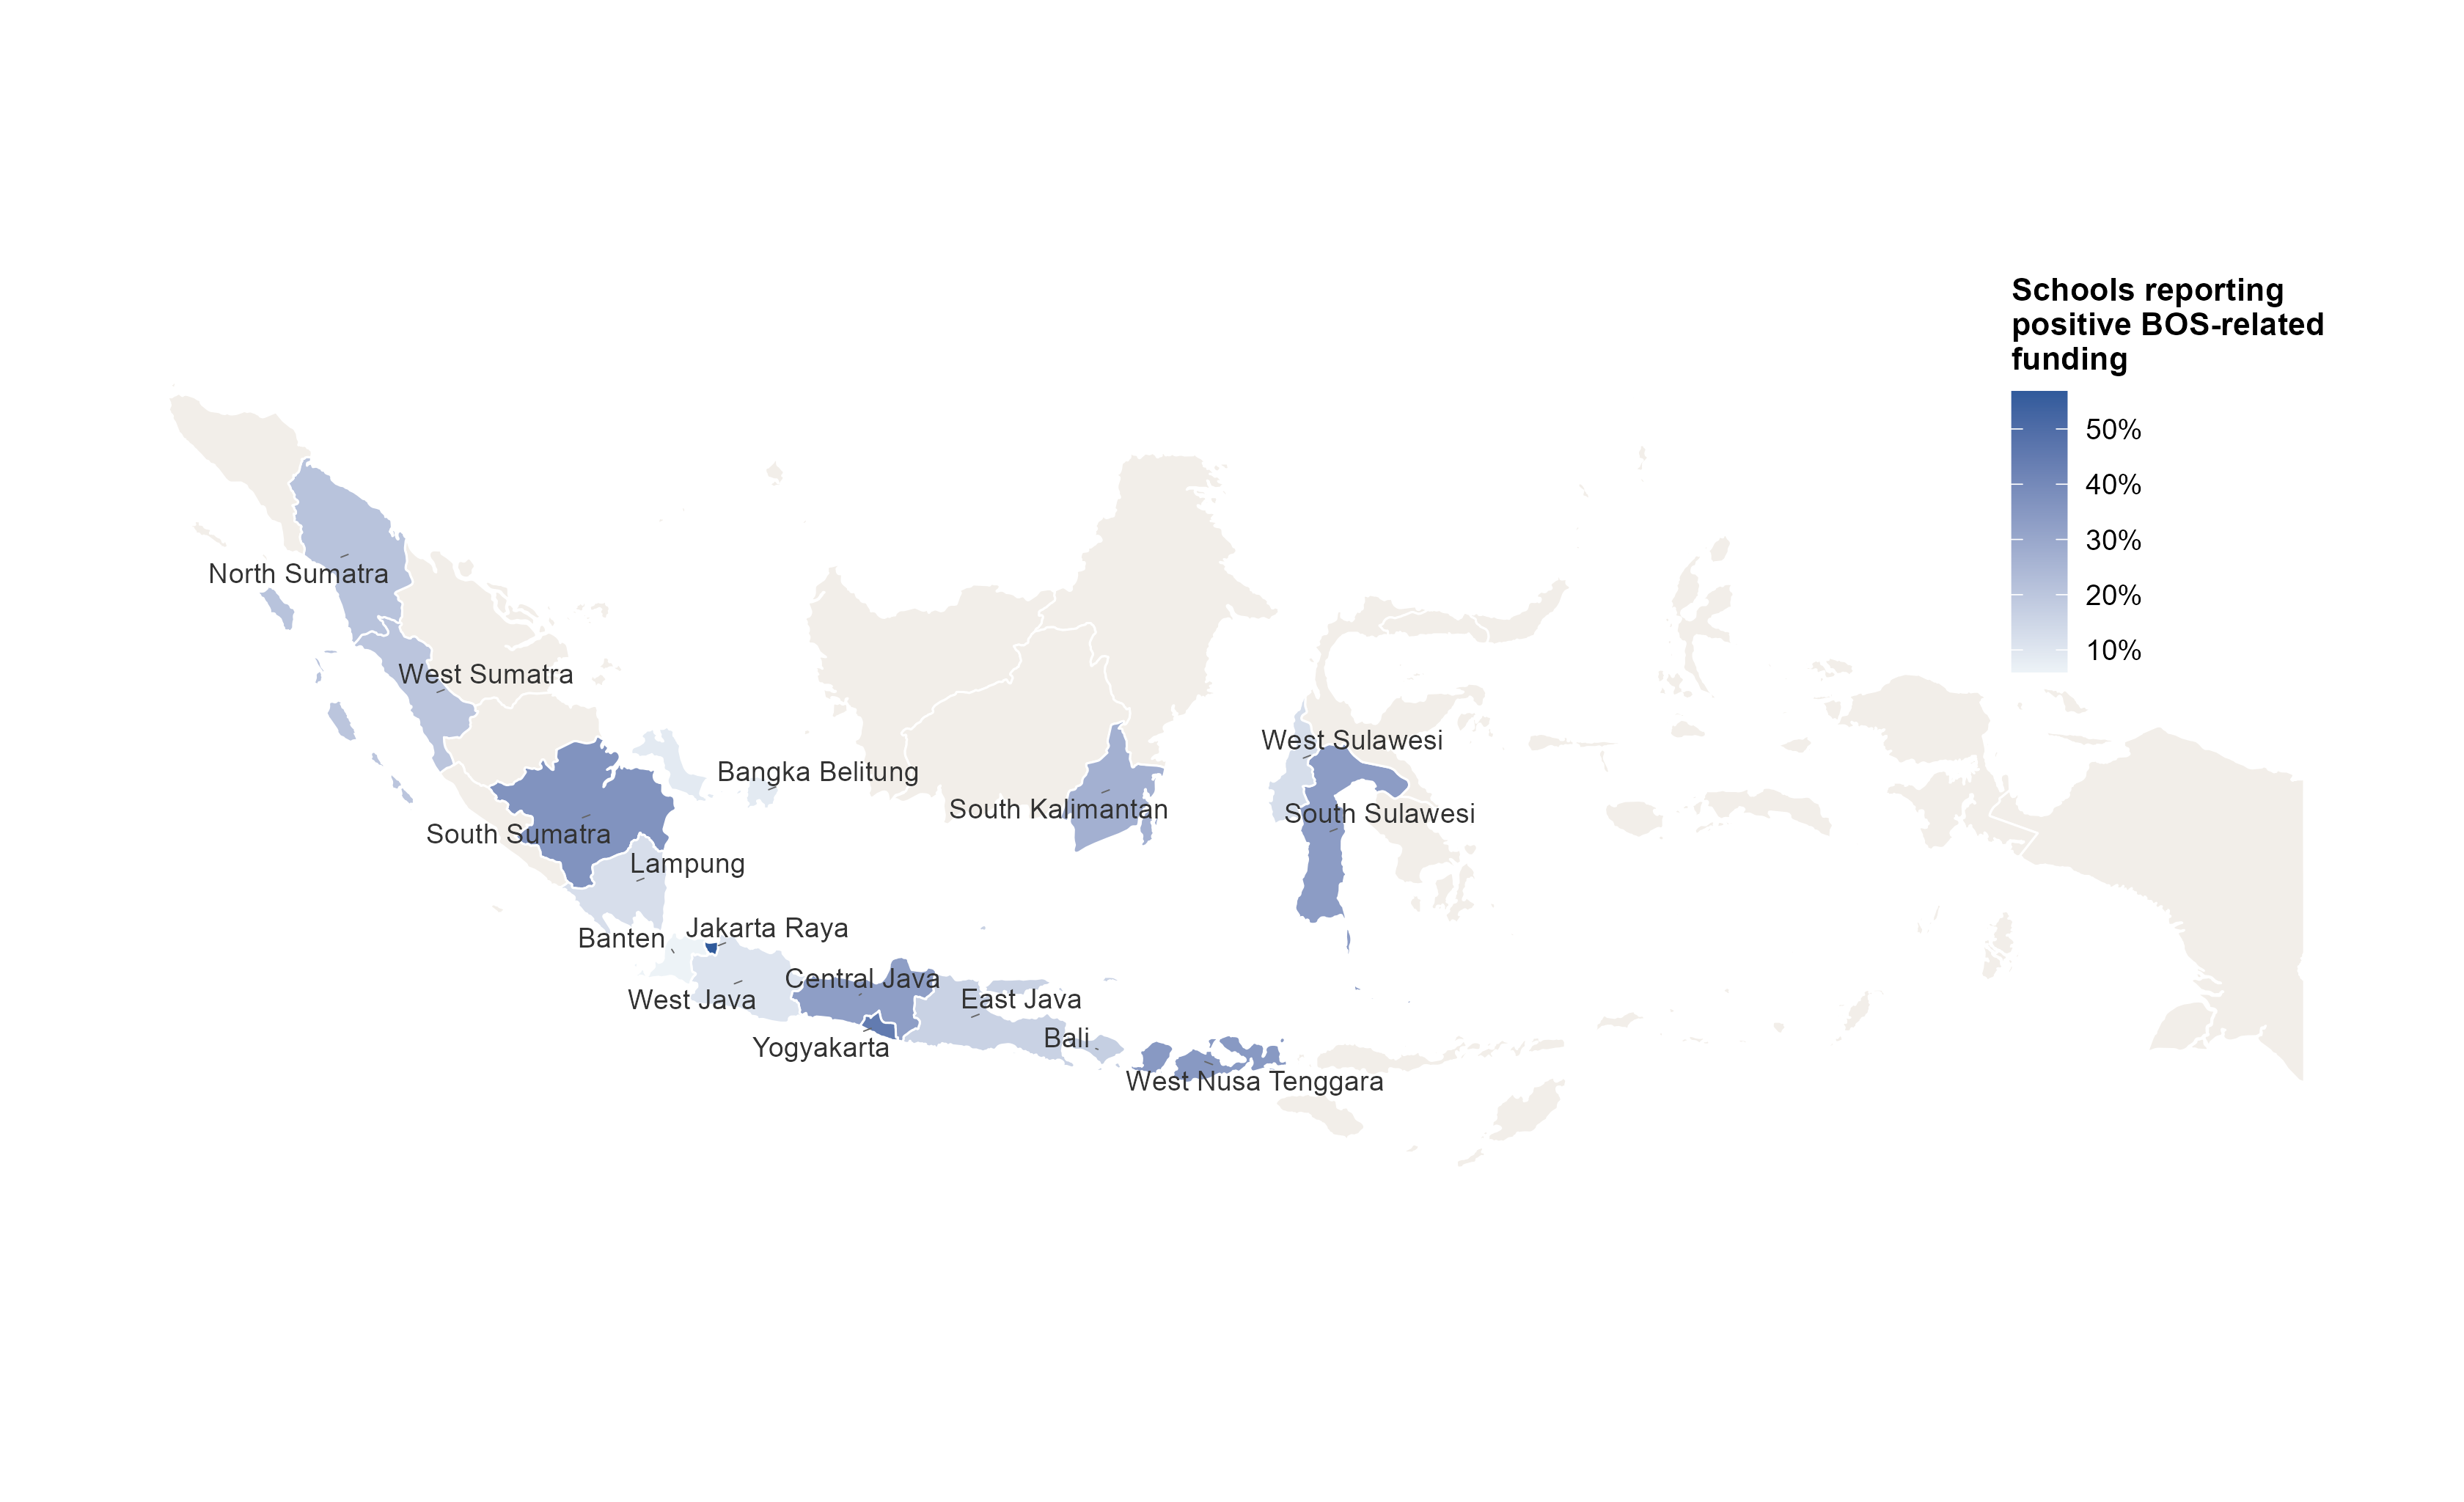
\includegraphics[width=0.95\textwidth]{indonesia_bos_intensity_2007_map_r.png}
\caption{Province-Level BOS Intensity Proxy in 2007}
\label{fig:intensity_map}
\end{figure}

A further measurement distinction is important for the educational outcomes. The completed-years measure captures completed years of schooling rather than current school level. It is constructed from the reported education level and the highest completed grade within that level. As a result, a child who has already entered senior high school but has not yet completed a senior-high grade may still have fewer than 10 completed years of schooling. The senior-high attainment indicator should therefore be interpreted as a threshold measure of completed attainment rather than as a direct measure of current senior-high enrollment.

\subsection{Main Specifications}
The preferred baseline specification uses the continuous potential-exposure measure and the binary 2007 high-intensity indicator. This version is easiest to interpret because the interaction coefficient represents how one additional potential BOS-exposed school year differs between higher- and lower-intensity provinces. To assess whether the result depends on this choice, I also estimate variants using binary cohort exposure and continuous intensity.

For the primary senior-high attainment outcome, I report four variants of the specification: binary exposure interacted with continuous intensity, binary exposure interacted with binary intensity, continuous exposure interacted with continuous intensity, and continuous exposure interacted with binary intensity. The same four variants are estimated for completed years of schooling as a secondary outcome. The main specification controls only for a female indicator, a fixed child characteristic that can vary across siblings within the same origin household. This adjustment accounts for gender differences in attainment while preserving a transparent within-household comparison.

\section{Results}
\subsection{Main Result}
Table \ref{tab:main_hs} reports the main estimates for senior-high attainment, which is the primary outcome of the thesis. The central parameter in each column is the interaction between child-specific BOS exposure and the province-level BOS intensity proxy. Across the four specifications, that interaction is positive. This pattern is consistent with the identifying idea of the paper: within the same origin household, siblings with greater potential BOS exposure tend to have somewhat better senior-high attainment outcomes when they are linked to provinces with stronger measured BOS intensity. At the same time, the estimates are not statistically significant at conventional levels, so the evidence should be read as suggestive rather than conclusive.

The clearest result appears in column (4), which is the preferred specification: continuous BOS exposure, measured as potential BOS-exposed school years, interacted with an indicator for provinces above the median of the 2007 intensity distribution. In this specification, the interaction coefficient is 0.010 and is statistically significant at the 10 percent level. Interpreted literally, this implies that an additional year of potential BOS exposure is associated with about a 1 percentage point higher probability of senior-high attainment in higher-intensity provinces relative to lower-intensity provinces. Relative to the control-group mean of 0.618, this is roughly 1.6 percent of the baseline attainment rate. Columns (1), (2), and (3) point in the same direction, but with wider standard errors.

The female coefficient is positive and statistically significant across specifications, at about 0.044. This means that, within the same origin household and conditional on the exposure and intensity terms, girls are about 4.4 percentage points more likely than boys to have completed at least 10 years of schooling. This coefficient should not be interpreted as evidence that BOS affected girls differently. Rather, it captures an average within-household gender difference in senior-high attainment and serves as a child-level control in the main specification.\footnote{Chapter 4.2 directly examines whether the BOS exposure-by-intensity relationship differs by child gender using triple-interaction specifications.}

The exposure main effect is small throughout. In the binary-exposure specifications, the higher-exposure cohort coefficient is positive but modest, and in the continuous-exposure specifications the coefficient on BOS years is 0.003. Because the household fixed effects absorb all shared family-level differences, these coefficients imply that exposure alone is not strongly associated with senior-high attainment within households. The main empirical pattern instead comes from the interaction term: the association between exposure and attainment is more favorable in places with stronger measured BOS intensity.
\clearpage
\begin{landscape}
    \begin{table}[!h]
\centering
\caption{Main Model: Effect on HS Attainment \label{tab:main_hs}}
\begin{threeparttable}
\footnotesize
\resizebox{\linewidth}{!}{%
\begin{tabular}[t]{@{}lcccc}
\toprule
 & (1) Bin Exp x Cont Int & (2) Bin Exp x Bin Int & (3) BOS Years x Cont Int & (4) BOS Years x Bin Int\\
\midrule
More Exposure (younger cohort) & 0.023 & 0.017 &  & \\
 & (0.031) & (0.021) &  & \\
More Exposure x BOS Intensity (2007 share) & 0.067 &  &  & \\
 & (0.108) &  &  & \\
More Exposure x High Intensity &  & 0.043 &  & \\
 &  & (0.029) &  & \\
Exposure (BOS years) &  &  & 0.003 & 0.003\\
 &  &  & (0.006) & (0.004)\\
Exposure (BOS years) x BOS Intensity (2007 share) &  &  & 0.020 & \\
 &  &  & (0.021) & \\
Exposure (BOS years) x High Intensity &  &  &  & 0.010*\\
 &  &  &  & (0.006)\\
Female & 0.043** & 0.044** & 0.043** & 0.044**\\
 & (0.019) & (0.019) & (0.019) & (0.019)\\
Num.Obs. & 2088 & 2088 & 2088 & 2088\\
R2 & 0.745 & 0.746 & 0.746 & 0.746\\
R2 Adj. & 0.556 & 0.557 & 0.557 & 0.558\\
Control Mean (treated = 0) & 0.618 & 0.618 & 0.618 & 0.618\\
Household FE & Yes & Yes & Yes & Yes\\
Controls & Female only & Female only & Female only & Female only\\
SE Cluster & Household & Household & Household & Household\\
\bottomrule
\end{tabular}
}
\begin{tablenotes}[para]
\item \textit{Notes: }
\item Cleaned HS models: all columns use household fixed effects and female as the only control. Binary intensity = 2007 median split. Continuous intensity = raw province-level 2007 BOS intensity share. Exposure in columns (3)-(4) is raw BOS years (not z-score). Control mean reports the lower-exposure cohort mean within the 2014 estimation sample. All standard errors are cluster-robust at household level.
\end{tablenotes}
\end{threeparttable}
\end{table}

\end{landscape}
\clearpage

Table \ref{tab:main_years} reports the corresponding results for completed years of schooling, which is treated as a secondary outcome. Here the interaction terms are small and statistically insignificant. The coefficient on the interaction between binary exposure and binary intensity in column (2) is -0.005, the corresponding continuous-exposure interaction in column (4) is -0.006, and the interaction with continuous intensity in column (3) is also imprecisely estimated. Taken together, these models do not show a robust relationship between greater BOS exposure and completed years of schooling by 2014.

The negative coefficients on the main exposure terms in Table \ref{tab:main_years} should not be interpreted as evidence that BOS reduced schooling. Completed years of schooling remains mechanically linked to age and lifecycle stage in the 2014 cross-section, and the more-exposed cohorts are younger by construction. By 2014, most children in the analytic cohorts are old enough for senior-high entry or attainment to be observed, but the youngest cohorts may still not have completed all schooling, making total completed years more sensitive to age. As a result, this outcome is less informative for the present design than the senior-high attainment threshold, which is why the latter remains the main outcome of interest.

Overall, the main results indicate a modest but suggestive positive relationship between BOS exposure and progression to senior high school in higher-intensity provinces. I emphasize senior-high attainment because it is the outcome most closely tied to the policy margin developed above: progression beyond compulsory basic education. The completed-years results are still reported as a secondary outcome, but they are less informative in the 2014 cross-section because completed schooling remains mechanically tied to age.

\clearpage
\begin{landscape}
    \begin{table}[!h]
\centering
\caption{Main Model: Effect on Years of Education \label{tab:main_years}}
\begin{threeparttable}
\footnotesize
\resizebox{\linewidth}{!}{%
\begin{tabular}[t]{@{}lcccc}
\toprule
 & (1) Bin Exp x Cont Int & (2) Bin Exp x Bin Int & (3) BOS Years x Cont Int & (4) BOS Years x Bin Int\\
\midrule
More Exposure (younger cohort) & -0.643*** & -0.754*** &  & \\
 & (0.186) & (0.134) &  & \\
More Exposure x BOS Intensity (2007 share) & -0.464 &  &  & \\
 & (0.663) &  &  & \\
More Exposure x High Intensity &  & -0.005 &  & \\
 &  & (0.183) &  & \\
Exposure (BOS years) &  &  & -0.116*** & -0.140***\\
 &  &  & (0.036) & (0.026)\\
Exposure (BOS years) x BOS Intensity (2007 share) &  &  & -0.113 & \\
 &  &  & (0.129) & \\
Exposure (BOS years) x High Intensity &  &  &  & -0.006\\
 &  &  &  & (0.036)\\
Female & 0.379*** & 0.378*** & 0.381*** & 0.378***\\
 & (0.124) & (0.124) & (0.124) & (0.124)\\
Num.Obs. & 2088 & 2088 & 2088 & 2088\\
R2 & 0.763 & 0.763 & 0.764 & 0.764\\
R2 Adj. & 0.587 & 0.587 & 0.588 & 0.588\\
Control Mean (treated = 0) & 10.860 & 10.860 & 10.860 & 10.860\\
Household FE & Yes & Yes & Yes & Yes\\
Controls & Female only & Female only & Female only & Female only\\
SE Cluster & Household & Household & Household & Household\\
\bottomrule
\end{tabular}
}
\begin{tablenotes}[para]
\item \textit{Notes: }
\item Cleaned years-of-education models: all columns use household fixed effects and female as the only control. Binary intensity = 2007 median split. Continuous intensity = raw province-level 2007 BOS intensity share. Exposure in columns (3)-(4) is raw BOS years (not z-score). Control mean reports the lower-exposure cohort mean within the 2014 estimation sample. All standard errors are cluster-robust at household level.
\end{tablenotes}
\end{threeparttable}
\end{table}

\end{landscape}
\clearpage

\subsection{Heterogeneous Treatment Effect}
Average effects can conceal meaningful subgroup differences, so I complement the main specification with two heterogeneity exercises that are especially relevant in this setting: child gender and parental education background. Following \citet{BitlerGelbachHoynes2006} and \citet{LehrerPohlSong2016}, the goal is not to build a separate identification strategy for each subgroup, but to assess whether the main within-household cohort-by-intensity pattern appears concentrated in particular types of families or children.

\subsubsection{Heterogeneity by Child Gender}
To examine whether the main relationship differs between girls and boys, I estimate a version of the preferred baseline specification that adds interactions with the female indicator. The estimating equation is:

\begin{equation}
\begin{aligned}
Y_{ih} =\;& \beta_{1} BOSYears_{i}
+ \beta_{2} \left(BOSYears_{i} \times HighIntensity_{r(h)}\right)
+ \beta_{3} Female_{i} \\
&+ \beta_{4} \left(BOSYears_{i} \times Female_{i}\right)
+ \beta_{5} \left(BOSYears_{i} \times HighIntensity_{r(h)} \times Female_{i}\right) \\
&+ \alpha_{h} + \varepsilon_{ih}
\end{aligned}
\end{equation}

In this specification, the coefficient of primary interest is $\beta_{5}$, which captures whether the interaction between BOS exposure and high regional intensity differs for girls relative to boys. Column (1) of Table \ref{tab:hte_main_hs} reports the result. The coefficient on $BOSYears_{i} \times HighIntensity_{h}$ is positive, at $0.009$, indicating that the baseline association between additional BOS exposure and senior-high attainment remains positive in higher-intensity provinces. However, the triple interaction with the female indicator is only $0.001$ with a standard error of $0.008$, and is therefore far from statistically significant. The coefficient on $BOSYears_{i} \times Female_{i}$ is also small, at $0.004$, and similarly imprecise. Taken together, these estimates provide no evidence that the association between BOS exposure and senior-high attainment differs meaningfully between girls and boys in the analytic sample.

This result suggests that the limited positive pattern in the main specification is not being driven disproportionately by one gender. The estimated interaction is broadly similar for girls and boys, although the estimates remain too imprecise to rule out smaller subgroup differences.

\subsubsection{Heterogeneity by Parents' Education}
A second heterogeneity dimension is parental education background. This exercise is motivated by the intergenerational mobility literature, which emphasizes the importance of family background, household resources, school finance, and school quality in shaping children's educational attainment and longer-run outcomes \citep{CholliDurlauf2022,AhsanEmranShilpi2024,Biasi2023}. In the present context, the question is whether the main BOS exposure-by-intensity relationship differs systematically between children from lower- and higher-parent-education households.

I define an indicator equal to one if the maximum observed parental education in the household is at least 10 completed years, and zero otherwise.

$$
ParentHS_{h} = 1\left\{\max(FatherEduc_{h}, MotherEduc_{h}) \geq 10\right\}
$$

\begin{table}[!h]
\centering
\caption{Heterogeneous Treatment Effects: HS Attainment \label{tab:hte_main_hs}}
\begin{threeparttable}
\footnotesize
\resizebox{\linewidth}{!}{%
\begin{tabular}[t]{@{}lcc}
\toprule
 & (1) Female HTE & (2) Parent HS HTE\\
\midrule
BOS Years x High Intensity & 0.009 & 0.012\\
 & (0.007) & (0.007)\\
BOS Years x Female & 0.004 & \\
 & (0.008) & \\
BOS Years x High Intensity x Female & 0.001 & \\
 & (0.008) & \\
BOS Years x Parent HS &  & -0.016**\\
 &  & (0.008)\\
BOS Years x High Intensity x Parent HS &  & -0.004\\
 &  & (0.011)\\
Female & 0.027 & 0.045**\\
 & (0.032) & (0.019)\\
Num.Obs. & 2088 & 2080\\
R2 & 0.746 & 0.747\\
R2 Adj. & 0.557 & 0.558\\
Outcome & HS attainment & HS attainment\\
Household FE & Yes & Yes\\
Heterogeneity Terms & Female interactions & Parent HS interactions\\
SE Cluster & Household & Household\\
\bottomrule
\end{tabular}
}
\vspace{0.5em}
\parbox{0.95\linewidth}{\footnotesize \textit{Notes:} All columns use the preferred main specification: BOS years x binary high-intensity indicator, with household fixed effects. Parent HS = 1 if the maximum observed parental education is at least 10 completed years. The coefficient on the triple interaction reports whether the BOS-years x high-intensity effect differs for girls or for children from higher-parent-education households.}
\end{threeparttable}
\end{table}


Because this parental-education measure is constant within household, its standalone main effect is absorbed by the household fixed effects. The estimating equation is therefore:

\begin{equation}
\begin{aligned}
Y_{ih} =\;& \beta_{1} BOSYears_{i}
+ \beta_{2} \left(BOSYears_{i} \times HighIntensity_{r(h)}\right) \\
&+ \beta_{3} \left(BOSYears_{i} \times ParentHS_{h}\right)
+ \beta_{4} \left(BOSYears_{i} \times HighIntensity_{r(h)} \times ParentHS_{h}\right) \\
&+ \gamma Female_{i} + \alpha_{h} + \varepsilon_{ih}
\end{aligned}
\end{equation}

In this specification, the coefficient of primary interest is $\beta_{4}$, which captures whether the interaction between BOS exposure and high regional intensity differs between children from higher- and lower-parent-education households.

Column (2) of Table \ref{tab:hte_main_hs} reports the result. The coefficient on $BOSYears_{i} \times HighIntensity_{h}$ is positive, at $0.012$, so the baseline interaction remains positive in higher-intensity provinces. However, the triple interaction between $BOSYears_{i}$, $HighIntensity_{h}$, and $ParentHS_{h}$ is $-0.004$ with a standard error of $0.011$, and is therefore not statistically significant. This suggests that the main BOS exposure relationship does not differ systematically by parental education background in the analytic sample.

The coefficient on $BOSYears_{i} \times ParentHS_{h}$ is $-0.016$ and statistically significant at the 5 percent level. This suggests that, outside the high-intensity interaction margin, the exposure slope may be somewhat smaller among children from households with higher parental education. However, this is not the main heterogeneity parameter of interest. The key point is that the preferred $BOSYears_{i} \times HighIntensity_{h}$ relationship is not meaningfully stronger or weaker across parental education groups.

Taken together, these estimates provide no evidence that the association between BOS exposure and senior-high attainment differs meaningfully by parental education background. The limited positive pattern in the main specification therefore appears broadly similar across households with lower and higher parental education, although the estimates remain imprecise.

\begin{figure}[H]
\centering
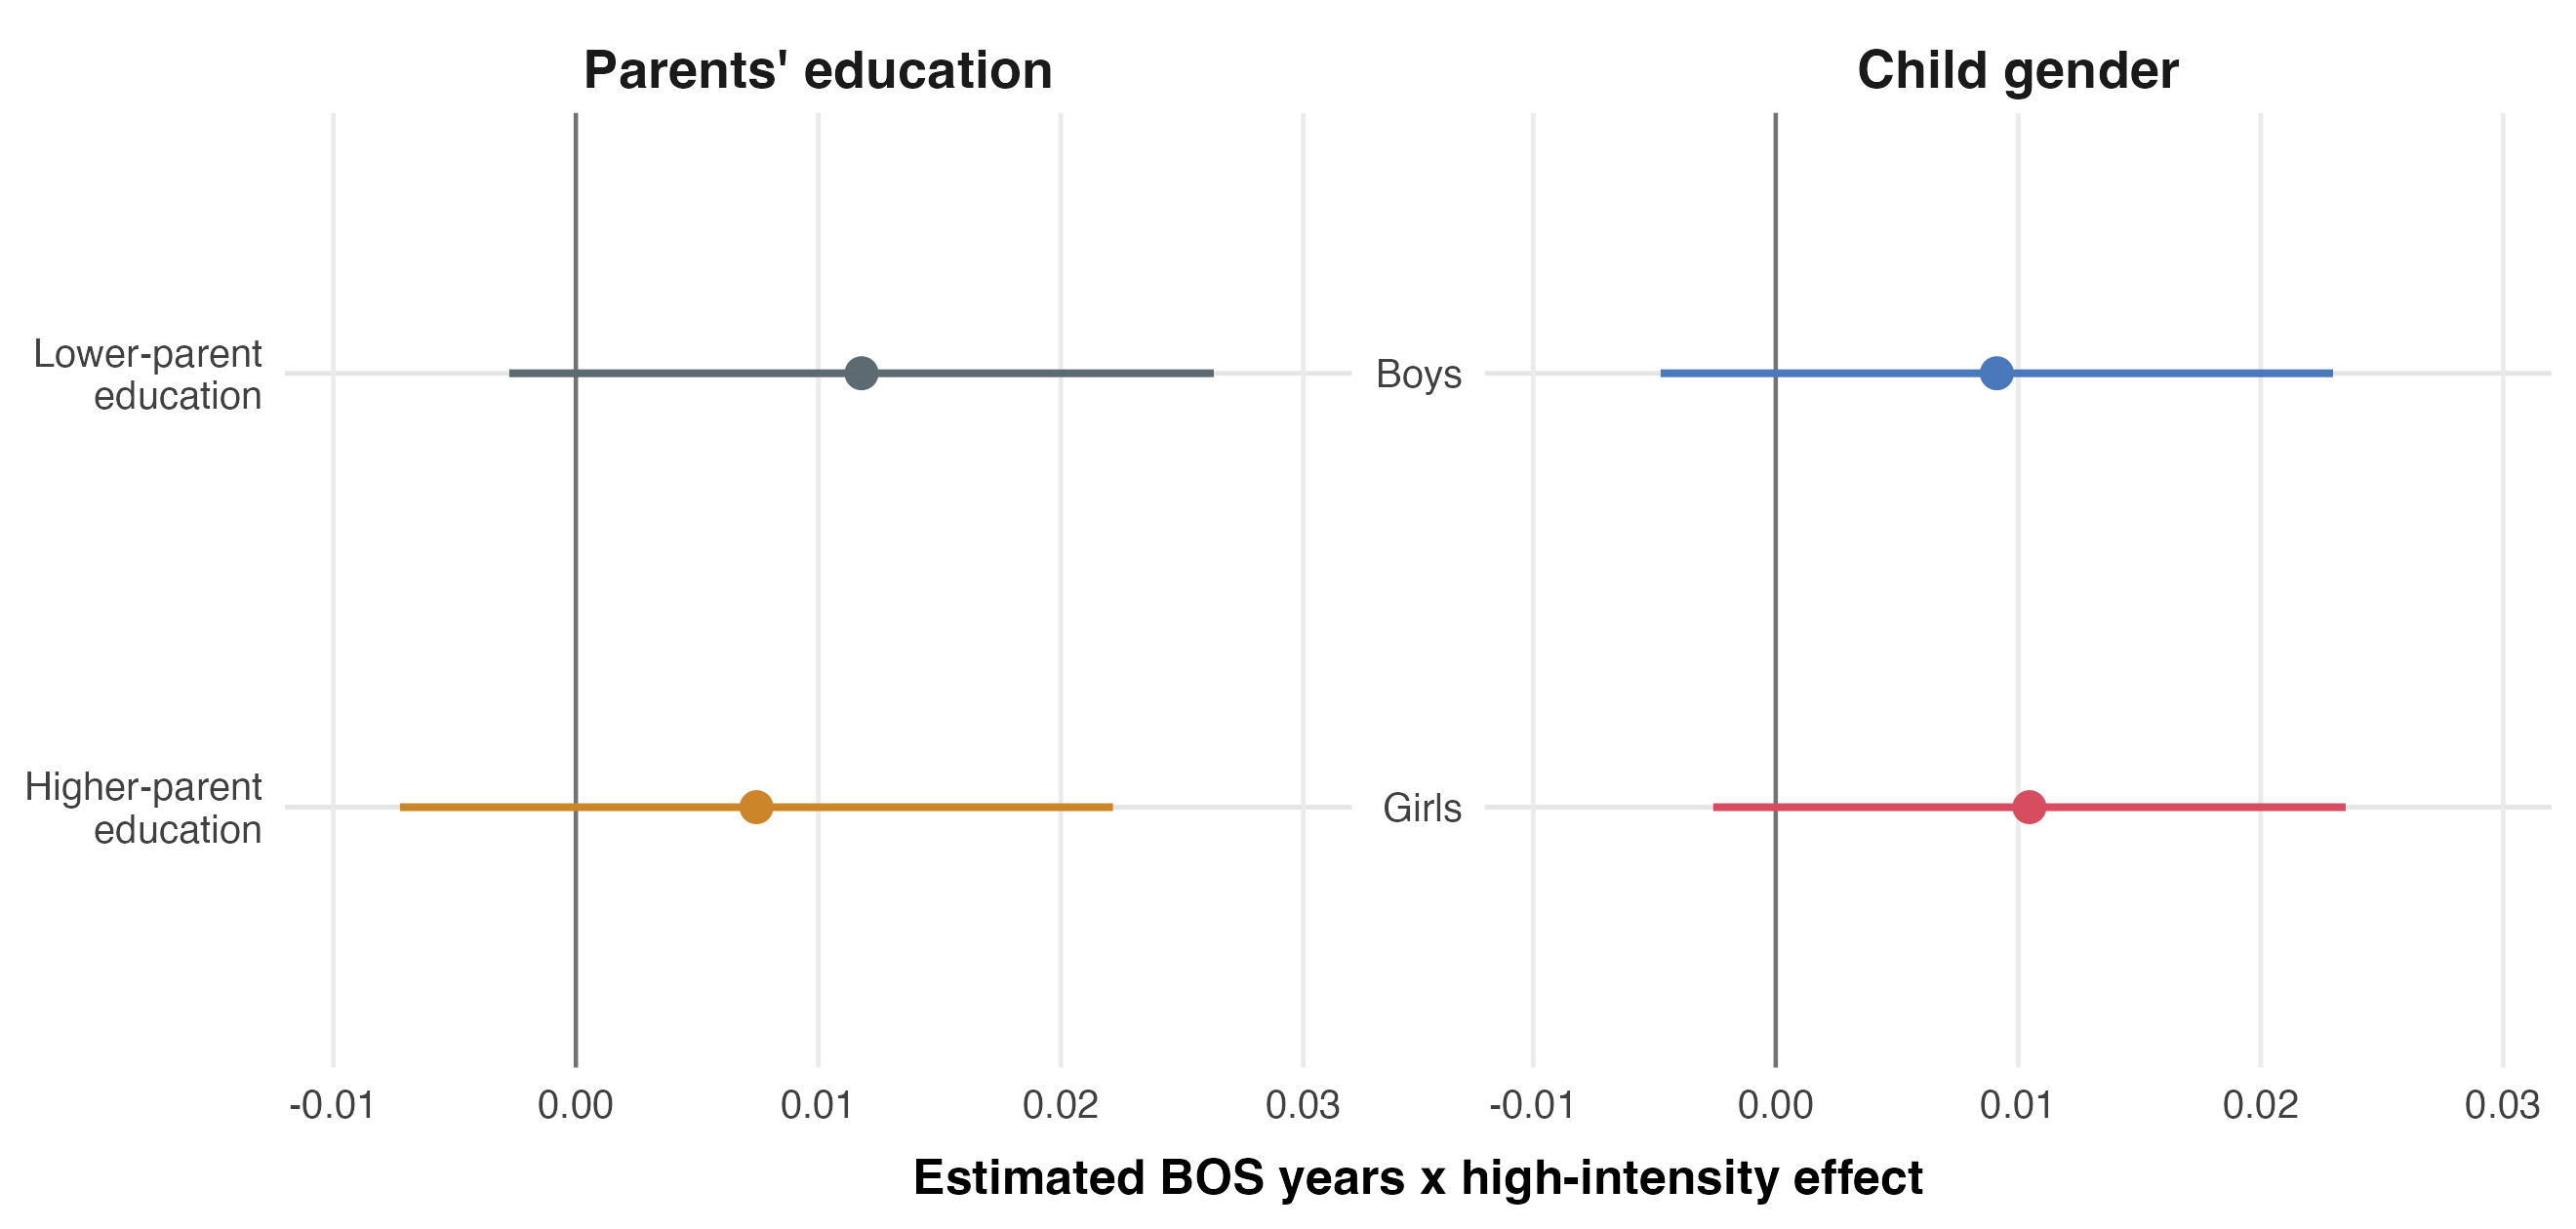
\includegraphics[width=0.95\textwidth]{heterogeneity_combined_thesis.png}
\caption{Estimated BOS Exposure Effects by Child Gender and Parental Education}
\label{fig:hte_combined}
\end{figure}

Figure \ref{fig:hte_combined} visualizes the heterogeneity estimates from Table \ref{tab:hte_main_hs}. Across both child gender and parental education background, the point estimates are positive but imprecise, and the confidence intervals overlap substantially. This reinforces the interpretation that the main BOS exposure-by-intensity relationship is not driven by a single subgroup. Hence, to put it more straightfoward, the figure provides no evidence of meaningful heterogeneity in the analytic sample.

\subsection{Sensitivity and Robustness Checks}
This subsection examines whether the preferred senior-high attainment result is sensitive to alternative ways of implementing the identification strategy. In causal research designs, it is standard to assess whether results are sensitive to alternative comparison windows and related design choices \citep{BertrandDufloMullainathan2004,XiaoLiZhao2017}. In the present 2014 analytic sample, birth years range from 1988 to 1997, so there are no cohorts older than the baseline lower-exposure group available for a separate placebo comparison. The sensitivity analysis therefore focuses on three design-based checks that remain close to the core specification: a narrower cohort window, an older-cohort restriction that reduces lifecycle concerns, and a stricter definition of high BOS intensity. I interpret these checks by focusing on the direction, magnitude, and precision of the estimates rather than on whether each alternative specification crosses a conventional significance threshold.

\begin{table}[H]
\centering
\caption{Sensitivity Checks for Senior-High Attainment\label{tab:robust_hs}}
\footnotesize
\resizebox{\linewidth}{!}{%
\begin{tabular}{@{}lcccc@{}}
\toprule
& (1) Baseline & (2) Narrow Window & (3) Older Cohorts Only & (4) Top-Tercile Intensity \\
\midrule
Exposure (BOS years) & 0.003 & 0.010 & 0.009 & 0.005 \\
& (0.004) & (0.009) & (0.006) & (0.004) \\
Exposure $\times$ Higher-Intensity Indicator & 0.010* & -0.005 & 0.005 & 0.007 \\
& (0.006) & (0.012) & (0.009) & (0.006) \\
Female & 0.044** & 0.012 & 0.042* & 0.043** \\
& (0.019) & (0.029) & (0.024) & (0.019) \\
Observations & 2,088 & 851 & 1,322 & 2,088 \\
Household FE & Yes & Yes & Yes & Yes \\
Controls & Female only & Female only & Female only & Female only \\
\bottomrule
\end{tabular}
}

\vspace{0.5em}
\parbox{0.95\linewidth}{\footnotesize Notes: All columns use the preferred 2014 household fixed-effects specification for the senior-high attainment indicator, with standard errors clustered at the household level. Column (2) restricts the sample to birth cohorts 1990--1992 and 1994--1995, excluding 1993 and the outer cohorts. Column (3) restricts the sample to birth cohorts 1988--1995 to reduce concern that the youngest cohorts had insufficient time to complete senior high school by 2014. Columns (1)--(3) define high intensity using the province-level 2007 median split of the BOS intensity proxy. Column (4) instead defines high intensity as the top tercile of the 2007 province intensity distribution. * $p<0.10$, ** $p<0.05$, *** $p<0.01$.}
\end{table}


Column (1) of Table \ref{tab:robust_hs} reproduces the preferred household fixed-effects specification for senior-high attainment. Column (2) narrows the cohort comparison to children born in 1990--1992 versus 1994--1995, while continuing to exclude the 1993 transition cohort. Under this tighter window, the interaction between BOS years and high intensity becomes negative and very imprecise ($-0.005$, s.e. $0.012$). This does not support a stable positive estimate once the cohort contrast is compressed, although it is also consistent with a substantial loss of precision when the effective sample is reduced.

Column (3) keeps the original identification logic but trims the youngest cohorts by restricting the sample to children born no later than 1995. This addresses the concern that the youngest children in the main sample may not yet have had enough time to cross the senior-high attainment threshold by 2014. The interaction estimate remains positive at $0.005$ (s.e. $0.009$), though smaller than in the baseline specification and not statistically distinguishable from zero. Column (4) redefines high intensity more strictly, using the top tercile rather than the median split of the 2007 province-level BOS intensity distribution. Under this alternative definition, the interaction coefficient remains positive at $0.007$ (s.e. $0.006$), but again imprecisely estimated.

Taken together, these checks suggest that the preferred estimate should be interpreted cautiously. The positive sign is preserved when excluding the youngest cohorts and when using a stricter top-tercile intensity definition, but the estimate becomes smaller and imprecise. The narrower cohort window produces a negative and highly imprecise estimate, suggesting that the result is sensitive when the cohort contrast and sample size are substantially reduced. I therefore interpret the evidence as suggestive of a positive BOS relationship at the senior-high margin, but not as a highly stable or precisely estimated treatment effect.

\section{Discussion, Policy Implications, and Limitations}
\subsection{Policy Implications}
The main policy lesson of this thesis is cautious but clear: if BOS affects educational progression, it appears to do so more strongly where implementation intensity is greater. The preferred estimates are positive only when child-specific exposure is interacted with a stronger measured funding environment, and even then the magnitude is modest. This pattern is consistent with policy reviews emphasizing that the practical performance of BOS depends on disbursement timing, administrative capacity, local oversight, and school-level implementation rather than on the national allocation rule alone \citep{WorldBank2008,WorldBank2014,SMERUUNESCO2024}. One implication is that improving implementation quality may be as important as changing the nominal scale of the subsidy.

A second implication concerns the policy margin at which BOS seems most relevant. The stronger evidence in this thesis comes from the senior-high attainment threshold, not from completed years of schooling. That distinction matters because the senior-high margin is closely related to continuation beyond compulsory basic education, where indirect costs, transition costs, and competing household demands may be more binding. The results therefore align with a broader literature showing that schooling subsidies and fee reductions can matter most at continuation margins where households still face important financial constraints \citep{GlewweMuralidharan2016,FilmerSchady2014,DufloDupasKremer2021}. For Indonesian policy, this suggests that BOS may be most effective when paired with complementary supports that reduce the non-tuition barriers to remaining in school.

The within-household perspective of the thesis also suggests that policy evaluation should not focus only on average differences across unrelated students or households. If subsidies relax household constraints without fully eliminating them, they may still affect how families allocate schooling resources across siblings. The evidence here does not identify large within-family redistributive effects, but it does suggest that sibling comparisons can add useful information about the margin at which broad schooling subsidies operate.

Finally, the findings point to an administrative-data agenda. The intensity measure used here is necessarily indirect because IFLS does not provide full BOS disbursement histories at the child-school level. Better integration of school-level BOS disbursement records, enrollment histories, and student progression outcomes would make it easier to distinguish whether local differences in BOS effectiveness arise from funding levels, timing of transfers, school management, or the interaction between school finance and household constraints.

\subsection{Limitations and Next Steps}
Several limitations shape the interpretation of the results. First, the province-level BOS intensity measure is constructed from IFLS school-facility information on BOS-related local operational funding rather than from administrative BOS allocation records. It is therefore a proxy for implementation intensity, not a direct measure of BOS spending received by each child's school. The estimates should accordingly be read as evidence based on variation within the IFLS analytic sample rather than as administrative-population estimates. Second, the main analysis uses a 2014 cross-section within a broader sibling panel. This is appropriate for the household fixed-effects design, but it also means that completed years of schooling remains mechanically linked to age and lifecycle stage, which is one reason the senior-high attainment threshold is the more informative outcome. Third, the main tables are unweighted. This choice keeps the focus on the within-household sibling comparison in the analytic sample, but it means the estimates should not be interpreted as weighted population averages for all Indonesian children.

Fourth, the sensitivity checks show that the preferred senior-high attainment result is not fully stable across alternative cohort definitions. Narrowing the cohort comparison or trimming the youngest cohorts reduces precision and attenuates the interaction estimate, while a stricter top-tercile intensity definition preserves the positive sign without yielding strong statistical precision. This pattern does not reverse the main finding, but it does imply that the evidence should be interpreted as suggestive rather than highly stable.

These limitations point naturally to next steps. One direction would be to link richer administrative information on BOS disbursements, school characteristics, and student histories so that treatment intensity could be measured more directly and at finer geographic resolution. A second would be to study longer-run outcomes beyond senior-high attainment, including tertiary enrollment and labor-market outcomes. A third would be to examine mechanisms more explicitly by combining school-finance data with household expenditure measures, fee information, or school-quality indicators.

More broadly, future work could extend the within-household perspective developed here. With larger samples or richer data, it would be useful to examine whether BOS mattered more in larger families, poorer households, or places with weaker school supply and administrative capacity. In that sense, the value of this thesis is not only in its point estimate, but also in showing that sibling-based exposure differences offer a useful way to study how broad education subsidies operate inside families.

\section{Conclusion}
This thesis studies whether siblings with greater cumulative exposure to Indonesia's BOS program attain more schooling and are more likely to reach senior high school than their less-exposed siblings. Using IFLS data, I combine within-household cohort differences in BOS exposure with cross-province variation in a BOS-related school-funding intensity proxy. The main empirical result is modest: in the preferred household fixed-effects specification, greater BOS exposure is positively associated with senior-high attainment in higher-intensity provinces, with an implied effect of about 1 percentage point per additional BOS-exposed year in a higher-intensity setting. By contrast, the results for completed years of schooling are weak and not robust, which is consistent with the concern that completed grades remain mechanically tied to age in the 2014 cross-section.

The sensitivity checks point in the same general direction, but they also underscore the fragility of the estimate. Narrowing the cohort window or removing the youngest cohorts makes the interaction smaller and statistically imprecise, while adopting a stricter top-tercile intensity definition preserves the positive sign but still leaves wide uncertainty. The evidence therefore supports a modest signal rather than a large effect that is invariant to reasonable alternative sample definitions.

Taken together, the findings suggest that broad schooling subsidies such as BOS may help children progress farther in the education system, but that any such effect depends importantly on local implementation intensity and the household constraints that shape schooling decisions within families. The evidence is suggestive rather than definitive, but it supports a useful substantive perspective: education policy should be evaluated not only by average differences across unrelated students or households, but also by how it changes schooling choices within families when resources remain limited.
\clearpage
\bibliographystyle{apalike}
\bibliography{references}
\clearpage
\section*{Appendix}
\begin{singlespace}

	This appendix provides supplementary details on variable construction, additional sensitivity checks for the completed-years outcome, and an exploratory heterogeneity check by female-headed household. These materials are intended to clarify measurement and robustness rather than introduce a separate main result.

	\begin{table}[H]
\centering
\caption{Appendix: Variable Construction\label{tab:appendix_variable_construction}}
\small
\begin{tabularx}{\textwidth}{@{}p{0.28\textwidth}X@{}}
\toprule
Variable & Construction and interpretation \\
\midrule
Senior-high attainment & Indicator equal to one if completed years of schooling are at least 10. This is the primary outcome and captures completed attainment at the senior-secondary threshold. \\
Completed years of schooling & Completed schooling years constructed from reported education level and highest completed grade within that level. This is a secondary outcome because it remains more mechanically related to age in the 2014 cross-section. \\
Potential BOS-exposed years & Count of potential school-age years between ages 6 and 15 that occurred after BOS began in 2005. This measure is based on birth year and policy timing, not verified school-level receipt. \\
Higher-exposure cohort & Indicator for children born in 1994--1997. Children born in 1988--1992 form the lower-exposure cohort, and the 1993 transition cohort is excluded. \\
BOS intensity share & Province-level share of sampled IFLS schools in 2007 reporting positive BOS-related local operational funding. This proxies for realized implementation intensity. \\
High-intensity province & Indicator equal to one for provinces above the median of the 2007 province-level BOS intensity share. \\
Parent HS & Indicator equal to one if the maximum observed parental education in the origin household is at least 10 completed years. \\
Female-headed household & Indicator equal to one if the origin household head is female in the baseline household-control file. \\
Origin household & Household identifier used to link siblings to the same family of origin. Household fixed effects are defined at this level. \\
\bottomrule
\end{tabularx}
\end{table}


	\begin{table}[H]
\centering
\caption{Appendix: Sensitivity Checks for Completed Years of Schooling\label{tab:appendix_robust_years}}
\footnotesize
\resizebox{\linewidth}{!}{%
\begin{tabular}{@{}lcccc@{}}
\toprule
& (1) Baseline & (2) Narrow Window & (3) Older Cohorts Only & (4) Top-Tercile Intensity \\
\midrule
Exposure (BOS years) & -0.140*** & -0.120** & -0.065 & -0.147*** \\
& (0.026) & (0.059) & (0.042) & (0.023) \\
Exposure $\times$ Higher-Intensity Indicator & -0.006 & -0.020 & -0.003 & 0.010 \\
& (0.036) & (0.073) & (0.055) & (0.037) \\
Female & 0.378*** & 0.500*** & 0.449*** & 0.378*** \\
& (0.124) & (0.176) & (0.153) & (0.124) \\
Observations & 2,088 & 851 & 1,322 & 2,088 \\
Household FE & Yes & Yes & Yes & Yes \\
Controls & Female only & Female only & Female only & Female only \\
\bottomrule
\end{tabular}
}

\vspace{0.5em}
\parbox{0.95\linewidth}{\footnotesize Notes: All columns use the preferred 2014 household fixed-effects specification for completed years of schooling, with standard errors clustered at the household level. Column (2) restricts the sample to birth cohorts 1990--1992 and 1994--1995, excluding 1993 and the outer cohorts. Column (3) restricts the sample to birth cohorts 1988--1995 to reduce concern that the youngest cohorts had less time to complete schooling by 2014. Columns (1)--(3) define high intensity using the province-level 2007 median split of the BOS intensity proxy. Column (4) instead defines high intensity as the top tercile of the 2007 province intensity distribution. * $p<0.10$, ** $p<0.05$, *** $p<0.01$.}
\end{table}


	\begin{table}[!h]
\centering
\caption{Appendix: Heterogeneity by Female-Headed Household \label{tab:appendix_female_head_hte}}
\begin{threeparttable}
\footnotesize
\resizebox{\linewidth}{!}{%
\begin{tabular}[t]{@{}lc}
\toprule
 & (1) Female-Headed HH HTE\\
\midrule
BOS Years x High Intensity & 0.008\\
 & (0.006)\\
BOS Years x Female-Headed HH & -0.015\\
 & (0.010)\\
BOS Years x High Intensity x Female-Headed HH & 0.012\\
 & (0.018)\\
Female & 0.044**\\
 & (0.019)\\
Num.Obs. & 2071\\
R2 & 0.745\\
R2 Adj. & 0.554\\
Outcome & HS attainment\\
Household FE & Yes\\
Heterogeneity Terms & Female-headed household interactions\\
SE Cluster & Household\\
\bottomrule
\end{tabular}
}
\vspace{0.5em}
\parbox{0.95\linewidth}{\footnotesize \textit{Notes:} This appendix table reports an exploratory heterogeneity check using the preferred main specification. Female-headed household is measured at the origin-household level; its standalone effect is absorbed by household fixed effects. The triple interaction reports whether the BOS-years x high-intensity relationship differs for children from female-headed households.}
\end{threeparttable}
\end{table}


\end{singlespace}
\end{doublespacing}
\end{document}
